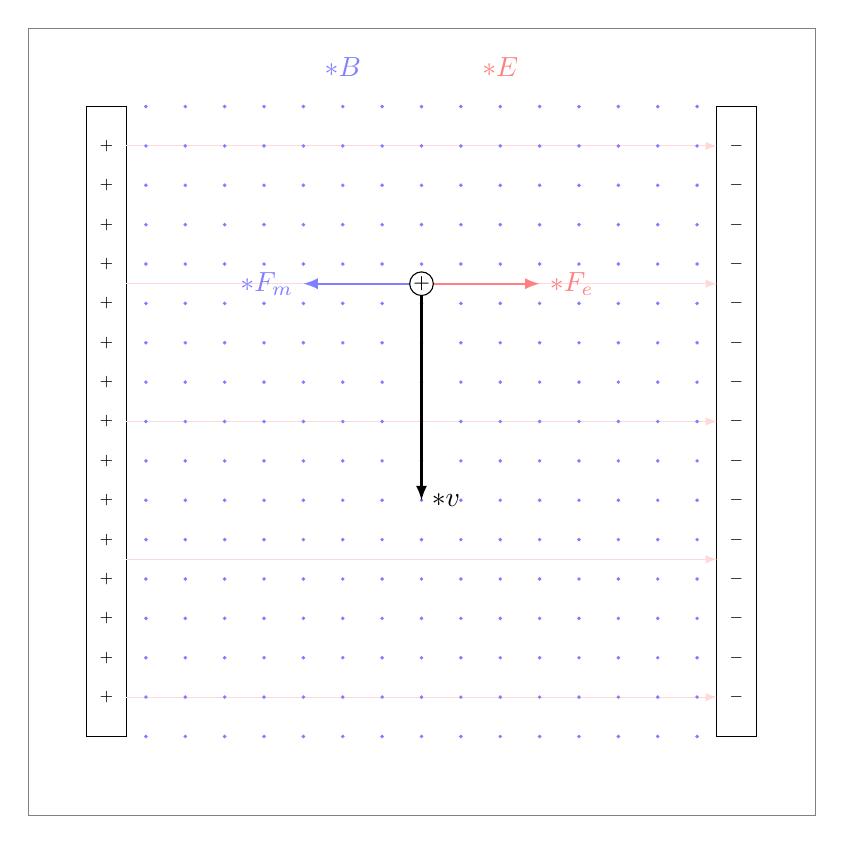
\begin{tikzpicture}[scale=1]
    \draw[gray,ultra thin] (-5,-5) rectangle (5,5);

    \draw (-4.25,4) rectangle (-3.75,-4);
    \draw (+4.25,4) rectangle (+3.75,-4);

    \foreach \y in {-3.50,-1.75,...,3.50}
    {
        \draw[red!15!white,-latex] (-3.75,\y)--(3.75,\y);
    }

    \foreach \x in {+3.50,+3.00,...,-3.50}
    {
        \foreach \y in {+4.00,+3.50,...,-4.00}
        {
            \fill[blue!50!white] (\x,\y) circle (0.025);
        }
    }

    \foreach \y in {3.50,3.00,...,-3.55}
    {
        \node at (-4,\y) {\tiny $+$};
        \node at (+4,\y) {\tiny $-$};
    }

    \draw[red!50!white,thick,-latex] (0,1.75)--(1.5,1.75) node[right] {$\vb*{F}_e$};
    \draw[blue!50!white,thick,-latex] (0,1.75)--(-1.5,1.75) node[left] {$\vb*{F}_m$};
    \draw[thick,-latex] (0,1.75)--(0,-1) node[right] {$\vb*{v}$};

    \node[red!50!white]  at (+1,4.5) {$\vb*{E}$};
    \node[blue!50!white] at (-1,4.5) {$\vb*{B}$};

    \draw[fill=white] (0,1.75) circle (0.15) node {\scriptsize $+$};
\end{tikzpicture}
